\documentclass[../main.tex]{subfiles}

\begin{document}

\section{Rate of Completions}

As learners engage in activities supported by a learning ecosystem, they will build
up a history of learning experiences. When the digital resources of that learning ecosystem
adhere to a framework dedicated to supporting and understanding the
learner, such as the Total Learning Architecture (TLA), it becomes
possible to retell their learning story through data and data visualization. One important aspect of
that story is the rate of completion\footnote{\label{defOfCompletion}
  Completion can be defined by the presence of the verb completed or by the presence of
  $\$.result.completion$ set equal to true. In this algorithm,
  completion is defined by the presence of the verb completed
  regardless of $\$.result.completion$. This decision affects how
  statements are retrieved and filtered. In the case where completion
  is defined by $\$.result.completion$, the query to the LRS would not
  include the verb paramater and there would need to be a filtering
  process which looks for the presence of $\$.result.completion$ =
  true} of the various digital resources within the learning
ecosystem.
\subsection{Ideal Statements}

In order to accurately portray the rates of completion, there
are a few base requirements of the data produced by a Learning Record
Provider (LRP). They are as follows:
\begin{itemize}
\item statements describing a learner completing an activity
  should\footnote{\label{verbIRICompletion} See footnote 4}
  use the verb $http://adlnet.gov/expapi/verbs/completed$
\item statements describing a learner completing an activity should
  report if the learner was successful or not via
  $\$.result.success$
\item statement describing a learner completing a scored activity
  should report the learners score via $\$.result.score.raw$,
  $\$.result.score.min$ and $\$.result.score.max$
\item activites must be uniquely and consistently identified across
  all statements
\item The time at which a learner completed a learning activity must be recorded
  \begin{itemize}
  \item The timestamp should contain an appropriate level of specificity.
  \item ie. Year, Month, Day, Hour, Minute, Second, Timezone
  \end{itemize}
\item statements describing a learner completing an activity should
  report the amount of time taken to complete the activity via $\$.result.duration$
\end{itemize}

\subsection{Input Data Retrieval}

How to query an LRS via a GET request to the Statements Resource via
curl. The following section contains the appropriate parameters with
example values as well as the curl command necessary for making the
request.\footnote{\label{refMoreLink2} See footnote
  1.}\footnote{\label{refnoZ2} See footnote
  2.}\footnote{\label{refallTime2} See footnote 3.}

\begin{lstlisting}[frame=single]
Verb = "verb=http://adlnet.gov/expapi/verbs/completed"

Since = "since=2018-07-20T12:08:47Z"

Until = "until=2018-07-21T12:08:47Z"

Base = "https://example.endpoint/statements?"

endpoint = Base + Verb + "&" + Since + "&" + Until

Auth = Hash generated from basic auth

S = curl -X GET -H "Authorization: Auth"
         -H "Content-Type: application/json"
         -H "X-Experience-API-Version: 1.0.3"
         Endpoint
\end{lstlisting}

\subsection{Statement Parameters to Utilize}

The statement parameter locations here are written in
\href{http://goessner.net/articles/JsonPath/}{JSONPath}. This notation
is also compatable with the xAPI Z notation due to the defined
hierarchy of components. Within the Z specifications, a variable name
will be used instead of the $\$$
\begin{itemize}
\item $\$.timestamp$
\item $\$.object.id$
\end{itemize}

\subsection{2018 Pilot TLA Statement Problems}

The initial pilot test data supports the core requirements of this
algorithm but completion statements only reports completion scores via
$\$.result.scaled$ instead of $\$.result.score.raw$,
$\$.result.score.min$ and
$\$.result.score.max$.\footnote{\label{scaledScores} The one potential
  issue with using scaled score is the
  calculation of scaled is not stricly defined by the xAPI
  specification but is instead up to the authors of the LRP. This
  results in the inability to reliably compare scaled scores across
  LRPs. if $\$.result.score.raw$ , $\$.result.score.min$ and
  $\$.result.score.max$ are reported for all questions, it becomes
  possible to reliably compare scores across LRPs by generating a
  scaled score in a consistent way.} Given that the offical 2018 pilot
test is scheduled to take place on July 27th, 2018, this section may
require updates pending future data review.

\subsection{Summary}

\begin{enumerate}
  \item Query an LRS via a GET request to the statemetns endpoint
    using the paramters verb, since and until.
  \item group statements by their $\$.object.id$
  \item select time range unit for use within rate calculation. Will
    default to day.
  \item determine the amount of time between the first and last instance of a $\$.object.id$ (in seconds) and divide it by the time unit. ie if the unit is minute, you would divide by 60.
  \item calculate the rate by dividing the count of a group (2) by the number of time units covered by the statements (4) so that the rate is the number of completions per activity per time unit.
\end{enumerate}

\subsection{Formal Specification}

\subsubsection{Basic Types}

$TIMEUNIT$ :== $\{second\} | \{minute\} | \{hour\} | \{day\} |
\{week\} | \{month\} | \{year\}$

\subsubsection{System State}

\begin{schema}{RateOfCompletion}
  Statements \\
  S_{completions} : \finset_1 \\
  S_{grouped},S_{timeunit}, S_{processed} : \finset \\
  \where
  S_{completions} = statements \\
  S_{grouped} = \{byId : \seq_1 statement\} \\
  S_{withRate} = \{byGroup: (\seq_1 statement, \nat)\} \\
  S_{processed} = \{rate : (id , \nat, TIMEUNIT)\}
\end{schema}
\begin{itemize}
\item The set $S_{completions}$ is a non-empty, finite set and is the
  component $statements$ which contains the results of the query to
  the LRS.
\item The sets $S_{grouped}$, $S_{withRate}$ and $S_{processed}$ are all finite sets
\item the set $S_{grouped}$ is a finite set of objects $byId$ which
  are non-empty, finite sequences of the component $statement$
\item the set $S_{withRate}$ is a finite set of objects $byGroup$ which
  are ordered pairs of non-empty, finite sequences of the component $statement$ and a natural number
\item the set $S_{processed}$ is a finite set of objects $rate$ where each
  contains the component $id$, a natural number and the type $TIMEUNIT$
\end{itemize}

\subsubsection{Initial System State}

\begin{schema}{InitRateOfCompletion}
  RateOfCompletion \\
  T : TIMEUNIT
  \where
  S_{completions} \not = \emptyset \\
  S_{grouped} = \emptyset \\
  S_{withRate} = \emptyset \\
  S_{processed} = \emptyset \\
  T = \{day\}
\end{schema}
\begin{itemize}
\item The set $S_{completions}$ is a non-empty set which contains the results of the GET request(s) to the LRS
\item The sets $S_{grouped}$ , $S_{withRate}$ and $S_{processed}$ are
  all initially empty
\item the variable T has the type $TIMEUNIT$ and the value $\{day\}$
\end{itemize}

\subsubsection{Calculate Rate}

\begin{schema}{IsoToUnix}
  convert : \finset_1 \fun \nat\#1 \\
  c? : \finset_1 \\
  c! : \nat\#1
  \where
  c! = convert(c?)
\end{schema}
\begin{itemize}
  \item The schema $IsoToUnix$ introduces the function $convert$ which
    takes in a finit set of one thing (a timestamp) and converts it to
    a single natural number.
  \item the purpose of this function is to convert an ISO 8601
    timestamp to the Unix epoch. The concrete definition of the conversion
    is outside the scope of this document
    \begin{itemize}
      \item The Unix epoch is the number of seconds that have elapsed
        since January 1, 1970 (midnight UTC/GMT), not counting leap seconds.
    \end{itemize}
  \end{itemize}

\begin{schema}{CalcRateByUnit}
  Statement \\
  IsoToUnix \\
  CountPerGroup \\
  unit? : TIMEUNIT \\
  s?,s! : \finset \\
  r : \nat \\
  rate : (\finset, TIMEUNIT) \fun \finset
  \where
  unit? \, = \,\{second\} \implies 1 \lor \{minute\} \implies 60
  \lor \{hour\} \implies 3600 \,\lor \\\t2 \{day\} \implies 86400 \lor
  \{week\} \implies 604800 \,\lor \\\t2 \{month\} \implies 2629743
  \lor \{year\} \implies 31556926 \\
  s? = \{g : seq_1 statement\} \\
  s! = rate(s?, unit?) \\
  s! = \{s : (g, r) \,|\, \forall g_{n}: g_{i}..g_{j} @ i \leq n \leq j @
  \exists \, s_{n} : (g_{n}, r_{n}) @ \\\t1
  r_{n} = count(g_{n}) \div ((convert(last~g_{n}.timestamp) - convert(head~g_{n}.timestamp)) \div unit?)\}
\end{schema}
\begin{itemize}
\item The schema $CalcRateByUnit$ introduces the function $rate$ where
  the input $s?$ is a set of objects $g$ which are each a non-empty,
  finite sequence of statements and the input $unit?$ represents a
  unit of time.
\item for every $g_{n}$ within the range $g_{i}..g_{j}$, there exists an associated object $s_{n}$ which is an orderd pair of $(g_{n}, r_{n})$ where $r_{n}$ is equal to the number of items within $g_{n}$ divided by the number of $unit?$s within the time range of $last~g_{n}.timestamp-head~g_{n}.timestamp$
\item the output of the function $rate$ is $s!$, the set of all $s_{n}$
\end{itemize}
$\\\\\\\\\\\\\\\\\\\\\\\\\\\\\\\\\\$ %%% keep header with z-schema
\subsubsection{Processes Results}
\begin{schema}{AggergateCompletionStatements}
  \Delta RateOfCompletion \\
  GroupByActivityId \\
  CalcRateByUnit \\
  grouped,processed,withRate : \finset \\
  r : \nat \\
  T? : TIMEUNIT
  \where
  T? = \{day\} \\
  grouped = \emptyset \\
  grouped' = group(S_{completions}) \\
  S_{grouped}' = S_{grouped} \cup grouped' \\
  withRate \subseteq S_{grouped}' \\
  withRate' = rate(withRate, T?) \\
  S_{withRate}' = withRate' \cup S_{withRate} \\
  processed \subseteq S_{withRate}' \\
  processed' = \{p: (id, r, T?) \,|\,
  \\\t3 \LET \{processed_{i}..processed_{j}\} == \{b_{i}..b_{j}\} @ \\\t3
  \forall b_{n} : b_{i}..b_{j} @ i \leq n \leq j @
  \exists \, p_{n} : (id_{n}, r_{n}, T?) @  \\\t3
  id_{n} = (head~(first~b_{n})).object.id \, \land \, \\\t3
  r_{n} = (second~b_{n})\} \\
  S_{processed}' = processed' \cup S_{processed}
\end{schema}

\begin{itemize}
\item The schema $AggergateCompletionStatements$ outlines how to calculate
  the rate of completion per $\$.object.id$ per $second|minute|hour|day|week|month|year$
  \begin{enumerate}
  \item $S_{grouped}'$ is the result of grouping the statements within $S_{completions}$ by their $\$.object.id$
  \item The groups from (1) are passed to the function $rate$ with the
    variable $T?$ which controls the unit of time, ie per day vs per week
  \item the result of (2) is then processed to create a triplet of
    $\$.object.id$, rate, unit of time for all unique $\$.object.id$
    within $S_{completions}$
\end{enumerate}
\end{itemize}

\subsubsection{Return}

\begin{schema}{ReturnAggergateCompletionStatements}
  \Xi RateOfCompletion \\
  AggergateCompletionStatements \\
  S_{processed}! : \finset
  \where
  S_{processed}! = S_{processed}
\end{schema}
\begin{itemize}
  \item The return value $S_{processed}!$ is equal to $S_{processed}$ after the operation described by $AggergateCompletionStatements$
\end{itemize}

\subsection{Pseudocode}

\begin{algorithm}[H]
  \SetAlgoLined
  \KwIn{$S_{completed}$, $timeUnit$}
  \KwResult{$ratePerObjTu'$}
  \emph{context = \{\}}\;
  \emph {ratePerObjTu = []}\;
  \While{$S_{completion} \not = \emptyset$}
  {\ForEach{$s \in S_{completion}$}
    {$id \leftarrow s.object.id$\;
      $ts \leftarrow convert(s.timestamp)$\;
      \eIf{$id \notin context$}
      {\bf do \\
        $times = [ts]$\;
        $context' \leftarrow \{id : times \}$\;
        $S_{completion}' \leftarrow S_{completion} \setminus s$\;
        recur $context', S_{completion}'$\;}
      {\bf do \\
        $times' \leftarrow context.id \cat ts$\;
        $context' \leftarrow \{id : times'\}$\;
        $S_{completion}' \leftarrow S_{completion} \setminus s$\;
        recur $context', S_{completion}'$\;}}}
  \ForEach {$k \in context'$}
  {$allTs \leftarrow context'.k$\;
    $totalDuration \leftarrow max(allTs) - min(allTs)$\;
    $totalCount \leftarrow count(allTs)$\;
    $rate \leftarrow totalCount \div (totalDuration \div timeUnit)$\;
    $subVec = [k, rate, timeUnit]$\;
    $ratePerObjTu' \leftarrow ratePerObjTu \cat subVec$\;
    {\bf recur} $ratePerObjTu'$\;}
 \Return $ratePerObjTu'$
  \caption{Rate of Completions}
\end{algorithm}
\begin{itemize}
\item Values from Z schemas are used within this pseudocode
\item the result of the algorithm is an array of arrays where each
  subarray contains a $statement.object.id$, the $rate$ and the
  $timeUnit$ used to calculate $rate$.
\end{itemize}
$\\$ %% header with text
\subsection{JSON Schema}

\begin{lstlisting}[]
{"type":"array",
   "items":{"type":"array",
      "items":[{"type":"string"}, {"type":"number"},
{"type":"string"}]}}
\end{lstlisting}

\subsection{Visualization Description}

The \textbf{Rate of Completions} visualization will be
a bar chart where the domain consists of $statement.object.id$ and the
range is a number greater than 0 (the rate of completions for that
$statement.object.id$). Every subarray within the array $ratePerObjTu$
will be a grouping within the bar chart. The pseudocode specifies an
input paramter $timeUnit$ which controls the calculation of the rate
(range of the visualization). $timeUnit$ could be per minute, per day,
per week, etc.

\subsection{Visualization prototype}

\pgfplotstabletypeset[string type]

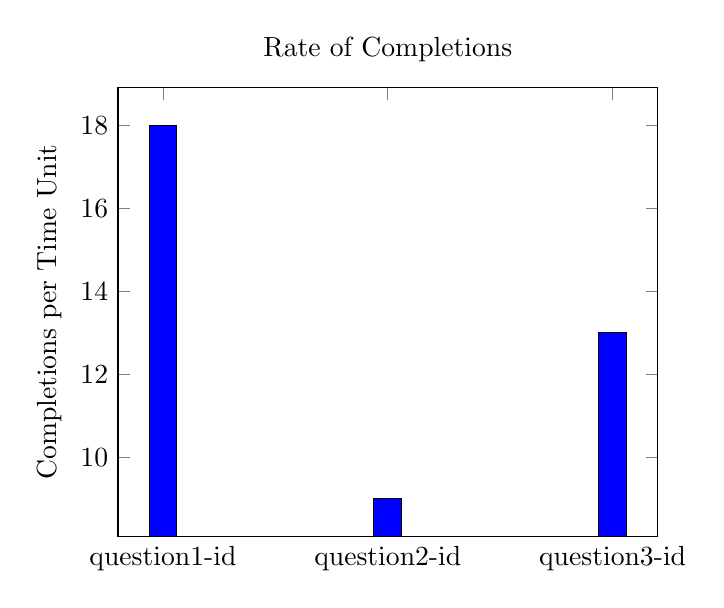
\begin{tikzpicture}
  \begin{axis}[
    title = Rate of Completions,
    ylabel = Completions per Time Unit,
    symbolic x coords={question1-id,question2-id,question3-id},
    xtick=data]
    \addplot[ybar,fill=blue] coordinates{
      (question1-id,18)
      (question2-id,9)
      (question3-id,13)
    };
  \end{axis}
\end{tikzpicture}

\subsection{Prototype Improvement Suggestions}
Additional features may be implemented on top of this base
specification but they would require adding aditional values to each
subarray returned by the algorithm. These additional values can be
retrieved via (1) performing metadata lookup within or independently of the
algorithm (2) by utilizing additional xAPI statement paramters and/or (3) by
performing additional computations. The following examples assume the
metadata is contained within each statement available to the algorithm.

\begin{itemize}
\item use $statement.object.definition.name$ instead of
  $statement.object.id$ for x axis label
\item populate a tooltip with the people who have completed the
  activity. This could also include the number of times they have
  completed it.
\item populate a tooltip with the breakdown of which devices or platforms the
  activity was completed on. This would require the device type or platform to be
  reported within $statement.context.platform$
\item populate a tooltip with the breakdown of percentage successful
  for all completions of the activty. This would require
  $statement.result.success$
\item populate a tooltip with the breakdown of scores earned (if
  appliciable) for the completions. This would require
  $statement.result.score.raw$, $statement.result.score.min$ and
  $statement.result.score.max$
\item populate a tooltip with the competency assocaited with the
  completed activities. The competency should be reported
  via $statement.context.contextActivities$
\item populate a tooltip with the average duration spent to reach
  completions. This would require $statement.result.duration$ to be reported.
\end{itemize}

\end{document}
